%!TEX root =../../../course-notes.tex
% ^ leave for LaTeXTools build functionality
\begin{applicationActivities}

\begin{observation}
There are two very simple kinds of separable ODEs.
\vfill
Equations of the form \(y'=f(x)\) can be solved immediately by integrating and produce explicit solutions.
\vfill
Equations of the form \(y'=f(y)\) are often impossible or difficult to solve explicitly.  They are called \term{autonomous} equations.
\end{observation}

\begin{activity}{10}
Consider the autonomous equation \[y'=y^2\].
\vfill
Suppose a solution goes through the point \(y(10)=50 \).  What can you say about \(y(11)\)?
\vfill
\begin{enumerate}[(a)]
\item \(y(10)<y(11)\)
\item \(y(10)=y(11)\)
\item \(y(10)>y(11)\)
\end{enumerate}
\end{activity}

\begin{activity}{10}
Consider the autonomous equation \[y'=y^2(y-2)\].

\begin{subactivity}
Draw a number line for \(y'\), indicating where it is positive or negative.
\end{subactivity}
\begin{subactivity}
What can you say about the long term behavior of a solution passing through \(y(4)=1\)?
\end{subactivity}
\end{activity}

\begin{definition}
The \term{phase line} is a useful way to visualize the long term behavior of an autonomous DE.
\vfill
For example, here is a phase line for the autonomous DE \(y'=y^2(y-2)\).

\begin{center}
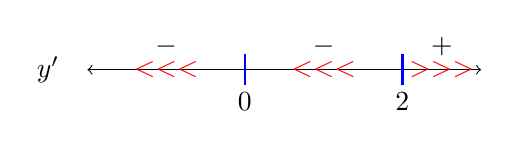
\begin{tikzpicture}
\node at (-2.5,0) {\(y'\)};
\draw[<->] (-2,0) -- (3,0);
\node at (-1,0.3) {\(-\)};
\node at (1,0.3) {\(-\)};
\node at (2.5,0.3) {\(+\)};
\draw[thick,blue] (0,-0.2) -- (0,0.2);
\node at (0,-0.4) {\(0\)};
\draw[thick,blue] (2,-0.2) -- (2,0.2);
\node at (2,-0.4) {\(2\)};
\node[red] at (-1,0) {\(<<<\)};
\node[red] at (1,0) {\(<<<\)};
\node[red] at (2.5,0) {\(>>>\)};
\end{tikzpicture}
\end{center}
\end{definition}

\begin{activity}{15}
Consider the autonomous equation \[y'=y(y+1)^2(y-2).\]

\begin{subactivity}
Draw a phase line.
\end{subactivity}
\begin{subactivity}
Describe the long term behavior of a solution passing through \(y(2)=-0.9999\).
\end{subactivity}
\begin{subactivity}
Describe the long term behavior of a solution passing through \(y(7)=-1.0001\).
\end{subactivity}
\begin{subactivity}
Describe the long term behavior of a solution passing through \(y(4)=-1\).
\end{subactivity}
\begin{subactivity}
Describe the long term behavior of solutions passing near the point \(y(3)=0\).
\end{subactivity}
\begin{subactivity}
Describe the long term behavior of solutions passing near the point \(y(11)=2\).
\end{subactivity}
\end{activity}

\begin{definition}
The \term{critical points} of an autonomous DE are the numbers that give rise to equillibrium solutions (e.g. \(0,-1,2\) in the previous problem).
\vfill
A \term{source} is an unstable equillibrium in which all nearby trajectories move away in the limit.
\vfill
A \term{sink} is a stable equillibrium in which all nearby trajectories approach the equillibrium in the limit.
\vfill
There are also unstable equillibria in which some nearby trajectories return, while others diverge, analagous to a saddle point.
\end{definition}

\begin{activity}{10}
Consider the autonomous equation \[y'=y^3(y-2)^2(y+1)(y-1).\]
\vfill
Find and classify all of the critical points.
\end{activity}


\end{applicationActivities}
